\section{Tags and Tag-Matching Metrics}

Rigorous comparison of disparate tag-matching schemes required careful standardization of tag representation, mutation, and match quality calculation.
This section summarizes the tag representation, mutation, and match quality calculation procedures used in our experiments and provides formal definition for each of the surveyed tag-matching schemes within that framework.

In all experiments, we used 32-bit bitstrings as tags.
Formally, we define a tag $t$ as a fixed-length binary vector,
\begin{align*}
t = \langle t_0, t_1, t_2, \dots, t_{n-2}, t_{n-1} \rangle
\end{align*}
where
\begin{align*}
\forall i, t_i \in \{0, 1\} \text{ and } n=32.
\end{align*}

In experiments where mutations were applied to tags, individual bits were toggled stochastically at a uniform per-bit rate.

We call an algorithm used to calculate the match quality between two tags a tag-matching metric.
A tag-matching metric takes two tags as operands and calculates a match distance between them.
Low match distance indicates a ``good'' or ``strong'' match.
High match distance indicates a ``poor'' or ``weak'' match.
For consistency between metrics, we bound all match distances so that a distance of 0 is the ``best'' possible match and a distance of 1 is the ``worst'' possible match.

Occasionally, it is convenient to discuss match quality in terms of closeness instead of distance.
So, we also employ a closeness terminology, which is inverse to the distance terminology.
Low match closeness corresponds a ``poor'' or ``weak'' match.
High match closeness corresponds to a ``good'' or ``strong'' match.
Again, for consistency, we restrict closeness values between 0 and 1.
A closeness of 0 corresponds to the ``worst'' possible match.
A closeness of 1 corresponds to the ``best'' possible match.

\begin{table*}[!htbp]
\begin{tabularx}{\textwidth}{l|X}
\textbf{Metric}       & \textbf{Description}                                                                                                                                        \\ \hline
Hash                  & SHA1 cryptographic hash of  concatenation of \texttt{tag\_0} and \texttt{tag\_1} \citep{eastlake2001us}                         \\ \hline
Hamming               & fraction of positions within \texttt{tag\_0} and \texttt{tag\_1} with mismatching bits                                                                         \\ \hline
Integer               & value added to the unsigned integer representation of \texttt{tag\_0} to reach representation of \texttt{tag\_1}, wrapping around if necessary \\ \hline
Bidirectional Integer & lesser of integer metric distances \texttt{d(tag\_0, tag\_1)} and \texttt{d(tag\_1, tag\_0)}                                                                \\ \hline
Streak                & ratio of lengths of contiguously matching and mismatching substrings \\ \hline
\end{tabularx}

% \begin{tabularx}{\textwidth}{l|X|X}
% \hline
% \textbf{Metric}       & \textbf{Commutative?} & \textbf{Multidimensional?} \\ \hline
% Hash                  & no                    & yes                        \\ \hline
% Hamming               & yes                   & yes                        \\ \hline
% Streak                & yes                   & yes                        \\ \hline
% Integer               & no                    & no                         \\ \hline
% Bidirectional Integer & yes                   & no
% \end{tabularx}

\caption{
Surveyed tag-matching metrics.
}
\label{tab:metrics}
\vspace{-6ex}
\end{table*}


We compared five tag-matching metrics: Hamming, hash, integer, bidirectional integer, and streak.
The Hamming and bidirectional integer metrics are included because of their ubiquity in artificial life systems.
The integer metric is included due to its use in seminal work exploring tag-matching in genetic programs \citep{spector2011tag, spector2011s,spector2012tag}.
The streak metric was proposed to model large-effect mutations observed in biology but, to our knowledge, has not yet been formally studied in an evolving system.
The hash metric is introduced in this work in order to investigate the implications of a completely geometrically-unstructured tag-matching scheme.
Table \ref{tab:metrics} compares summary descriptions for each metric.

% Full mathematical definitions and implementation details appear in \href{doi.org/10.17605/OSF.IO/GW5MC}{supplementary material} \citep{Moreno_Ofria_2020}.

Sections \ref{sec:hamming}, \ref{sec:hash}, \ref{sec:integer}, \ref{sec:bidirectionalinteger}, and \ref{sec:streak} provide formal definitions for each metric.

\subsection{Hash Metric} \label{sec:hash}

To our knowledge, the hash metric is original to this work.
The metric produces an arbitrary, but deterministic, match distance between any two tags.
In other words, the tag matching space is completely unstructured.
We include it primarily to serve as a control.

The hash metric calculates match distance via a cryptographic hash of tags $t$ and $u$.
First, we concatenate $t$ and $u$ into a double-width bitstring $v$ such that
\begin{align*}
v = \langle t_0, t_1, t_2, \dots, t_{n-2}, t_{n-1}, u_0, u_1, u_2, \dots, u_{n-2}, u_{n-1} \rangle
\end{align*}

Then, we use the OpenSSL library to generate a \texttt{std::string} digest of $v$.
We then apply \texttt{std::hash} to map this digest to a \texttt{std::size\_t}, $v'$.
Finally, we perform a floating point division to compute the matching distance as $d(t, u) = v' / \hat{V}$ where $\hat{V}$  denotes the maximum representable \texttt{std::size\_t} value.

Note that this metric is not commutative.
As noted above, however, tag-matching systems inherently distinguish queries and operands.
So, an ordering within each pair of tags processed in a tag-matching system will be well-defined.
We use the convention of ordering the operand tag after the query tag when concatenating the tags' bit representations.

\subsection{Hamming Metric} \label{sec:hamming}

The Hamming metric computes match distance as the fraction of positions between tags $t$ and $u$ with mismatching bits.
Formally, for $n$-bit bitstring tags,
\begin{align*}
d(t, u)
= \frac{
  \#\{ i : t_i \neq u_i, i=0, \dots ,n-1\}
}{
  n
}.
\end{align*}

As an example, consider eight bit tags $t = \langle 1, 0, 0, 1, 0, 0, 1, 1 \rangle$ and $u = \langle 0, 0, 1, 0, 0, 0, 1, 1 \rangle$.
Sites 1, 4, 5, 6, 7, and 8 match.
Sites 0, 2, and 3 mismatch.
Because 3 sites mismatch, the Hamming metric would compute match distance as $3 / 8 = 0.375$.

This metric is based on \cite{lalejini2019else}, originally after \cite{hamming1950error}.

\subsection{Integer Metric} \label{sec:integer}

The integer metric computes match distance between tags $t$ and $u$ by counting upwards from $t$ until $u$ is reached.
If necessary, the counting process wraps around at $2^n$.

To accomplish this, the integer metric must interpret bitstring tags $t$ and $u$ as unsigned integers.
We use a standard representation,
\begin{align*}
f(t)
= \sum_{i=0}^{n-1} t_i \times 2^i.
\end{align*}

Formally, the integer metric computes distance between $n$-bit bitstring tags as,
\begin{align*}
d(t, u) = \frac{\Big(f(u) - f(t)\Big) \mod 2^n}{2^n}.
\end{align*}

Inclusion of this metric is motivated by \cite{spector2011tag}, who used positive integers between 0 and 100 to name referents.
Queries matched to the referent that had the next-larger value, wrapping around from 100 back to 0.

Like the hash metric, this metric is not commutative.
We adopt the convention of using the query tag as $t$ and the operand tag as $u$.

\subsection{Bidirectional Integer Metric} \label{sec:bidirectionalinteger}

The bidirectional integer metric computes match distance between tags $t$ and $u$ by counting from $t$ to $u$.
The count from $t$ to $u$ ascends or descends, whichever is shorter.
If necessary, the count wraps around at $0$ and $2^n$.

The bidirectional integer metric interprets bitstring tags $t$ and $u$ as unsigned integers using the same mapping, $f$, as the integer metric.

Formally, the bidirectional integer metric computes distance between $n$-bit bitstring tags as,
\begin{align*}
d(t, u) =
  \frac{\min \Big(f(u) - f(t)  \mod 2^n, f(t) - f(u) \mod 2^n \Big)}{2^n}. \\
\end{align*}

We included this metric to contrast with the integer metric. In particular, we wished to shed light on any consequences of its asymmetry and discontinuity.
In figure axes and legends with tight space constraint, we refer to this metric as ``Integer (bi).''

\subsection{Streak Metric} \label{sec:streak}

The streak metric computes match distance between bitstring tags $t$ and $u$ as a ratio of lengths of contiguously matching and mismatching substrings within those tags.

Formally, we can compute the greatest contiguously-matching length of $n$-long bitstrings $t$ and $u$ as,
\begin{align*}
m(t, u) = \max\Big(\{i - j \forall i, j \in 0..n-1 \mid \forall q \in i..j, t_q = u_q \}\Big).
\end{align*}

Likewise, the greatest contiguously-mismatching length can be computed as,
\begin{align*}
n(t, u) = \max\Big(\{i - j \forall i, j \in 0..n-1 \mid \forall q \in i..j, t_q \neq u_q \}\Big).
\end{align*}

As proposed in \cite{downing2015intelligence}, the streak metric computes distance between $n$-bit bitstring tags $t$ and $u$ as,
\begin{align*}
d'(t, u)
= \frac{p'(n(t,u))}{p'(m(t,u)) + p'(n(t,u))}.
\end{align*}
where $p(k)$ approximates the probability of a contiguous match at least $k$ bits long between two randomly sampled bitstring tags.

\cite{downing2015intelligence} derives
\begin{align*}
p'(k)
= \frac{n - k + 1}{2^k}.
\end{align*}

However, this formula is subtly flawed.
For instance, the probability of a $0$-bit match according to this formula would be computed as $p'(0) = \frac{n - 0 + 1}{2^0} = n + 1$.
This is clearly impossible --- it would imply $p'(0) > 1 \forall n > 0$.

Although correct probabilities can be calculated via dynamic programming, $p'$ provides a useful approximation.
For computational efficiency and consistency with the existing literature, we use the math proposed in \citep{downing2015intelligence} but clamp edge cases between 0.0 and 1.0.
Additionally, because Downing uses the match closeness convention where a perfect match is scored 1.0, we subtract from 1 to convert to match distance.
This yields the corrected streak metric $d$ used in this work,
\begin{align*}
d(t, u) = 1 - \max\Big( \min( d'(t, u), 1), 0 \Big).
\end{align*}

Downing motivates the streak metric by analogy to the biochemistry of enzyme-ligand binding.
In motivating the metric, Downing reports mutational walk experiments that show it to exhibit greater robustness compared to integer and Hamming metrics.
However, it is not demonstrated in an evolving system.
To our knowledge, no further work on this metric has been published.
(Although, through personal communication, we learned of some unpublished work applying the metric in a neuroevolution system.)


\subsection{Match Distance Uniformification}
\label{sec:uniformification}

\begin{figure}
\begin{center}

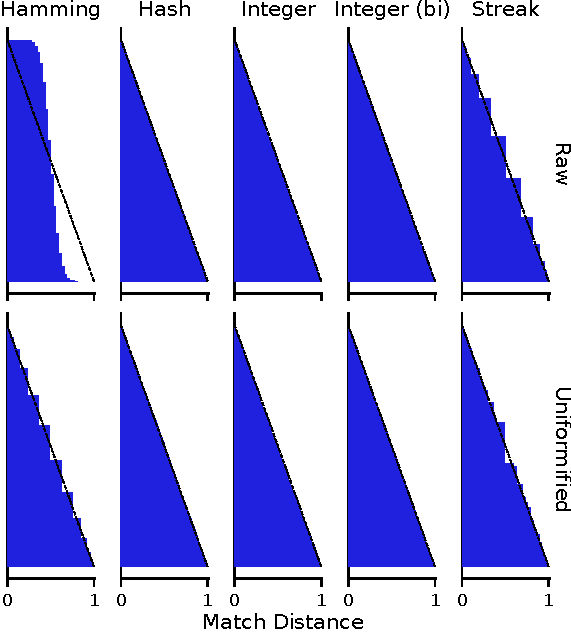
\includegraphics[width=\columnwidth]{img/uniformification/bitweight=0dot5+seed=1+title=low-score-distribution+_data_hathash_hash=75684cf1e73fb7f1+_script_fullcat_hash=d4b3b5e14a0d1350+ext=}
\caption{
Distance distributions of metrics before and after uniformification.
Dashed line indicates an ideal uniform distribution.
}
\label{fig:uniformification}

\end{center}
\end{figure}


For consistency of implementation and interpretation, all metrics output tag-matching distances between 0.0 (a ``perfect'' match) and 1.0 (a ``worst'' match).

However, the distribution of tag-match distances within this range may vary substantially between metrics.
For example, the probability of a match distance $<1/32$ between two randomly-sampled bitstring tags is $1/32$ under the hash metric but $1/2^{32}$ under the Hamming metric.

In order to ensure an intuitive interpretation of match distances that was consistent across all tag-matching metrics, we normalized metrics' match distances so that the distances between pairs of randomly generated tags would follow a uniform distribution between 0.0 and 1.0.
We call this process ``uniformification.''
In this discussion, we refer to match distance before uniformification as ``raw.''

For example, two tags with a 0.01 uniformified match distance would be better-matched than 99\% of randomly-generated tag pairs.
Additionally, in situations where raw match distance plays a mechanistic role (for example, probabilistic matching or threshold-based cutoffs), this transformation ensures consistency across metrics.

We performed this uniformification independently for each tag-matching metric using the following Monte Carlo approximation method.
\begin{enumerate}
\item We sampled 10,000 pairs of randomly-generated tags.
\item We calculated raw match distance between each pair of generated tags using the chosen tag-matching metric.
\item We organized these 10,000 sampled raw match distances into a list in ascending order.
\item To ensure coverage of the entire $[0.0,1.0]$ interval of valid tag match scores, we bookended the sorted list of raw match distances with 0.0 and 1.0.
\item We associated each list entry with its percentile ranking within the list.
\begin{enumerate}
    \item i.e., the best-matching 0.0 match distance was associated with the percentile ranking 0.0,
    \item the median match distance was associated with the percentile ranking 0.5, and
    \item the worst-matching 1.0 match distance was associated with the percentile ranking 1.0.
\end{enumerate}
\item For subsequent tag match distance calculations during the experiment, we performed a lookup on this list.
\begin{itemize}
    \item If a single exactly-identical raw match distance existed in the list, we returned its percentile ranking as the uniformified match distance.
    \item If two or more exactly-identical raw match distances existed in the list, we returned the mean percentile ranking of these entries as the uniformified match distance.
    \item If no exactly-identical raw match distance existed in the list, we linearly interpolated between the next-largest and next-smallest list entries' percentile rankings.
\end{itemize}
\end{enumerate}
Figure \ref{fig:uniformification} compares the distribution of match distances between randomly-sampled tags before and after this uniformification process across tag-matching metrics.

Error in the Monte Carlo approximation of the percentile for any raw match score is distributed binomially.
With 10,000 samples, absolute error at the 50th percentile can be bounded below 0.01 match distance units with 95\% confidence and below 0.012 match distance units with 99\% confidence.
% https://www.wolframalpha.com/input?i=binomial+distribution%2810000%2C+0.5%29+percentile
Absolute error at the 1st percentile can be bounded below 0.0017 match distance units with 95\% confidence and below 0.0024 match distance units with 99\% confidence.
% https://www.wolframalpha.com/input?i=binomial+distribution%2810000%2C+0.99%29+percentile
(With five independent uniformification processes, 99\% confidence per metric translates to 95\% confidence over all metrics under Bonferroni correction.)

All work reported here employed match distance uniformification.
A single match distance lookup table was used across all experiments with each metric.
Note that match distance uniformification has no effect in experiments where tag-matching derives exclusively from relative ordering with no absolute match distance effect (i.e., evolutionary experiments with the graph-matching and changing-signal tasks introduced later on).

\subsection{Note on Tag Alphabet}

For tractability and consistency, this work exclusively considers strings composed from the binary alphabet $\{0, 1\}$.
However, we expect that most geometric, variational, and evolutionary properties of the metrics studied are not fundmaentally tied to the particular use of the binary alphabet.

We suspect that the surveyed integer metrics under the existing bitstring representation should behave effectively indistinguishably from a continuous-valued (i.e., floating point) representation.
Due to the uniformification process performed, both would be effectively rescaled to the range $[0, 1]$.
With a precision of $1/2^{32}$ --- tighter than $10^{-9}$ --- the 32-bit tags used should exhibit near-undetectable granularity, especially given the relatively small pools of query and operand tags used in our experiments.

However, it is important to note that the bit flip mutation operator used in our experiments induces a rougly exponential distribution of effect size, which might otherwise be an unusual choice when working with a continuous-valued tag system.
We unpack this issue in greater detail in Section \ref{sec:variational}.

Alternate alphabet choice would have a minimal effect on the streak metric.
Imagine, for example, using a four-valued alphabet instead of the existing two-valued binary alphabet.
Any character in that four-valued alphabet could be encoded by a pair of binary digits.
So, the existing bitstring representation for tags could be preserved and adjustment instead made to the match distance metric to count only entirely-matching (or mismatching) pairs of bits as contributing to a streak.
The significance of this effect would depend on typical streak length and, of course, for large alphabets this truncation effect would eventually become overwhelming.

Increased alphabet size might have a more nuanced effect on the Hamming metric.
Under the binary alphabet, every mutation affects a tag's match distances to all other tags --- no mutation is neutral.
However, with a larger alphabet size this would no longer be the case.
As with the streak metric, increased alphabet size would introduce effects from coarsened granularity, with the magnitude of these effects eventually becoming overwhelming under large alphabets.

We do not fully explore the possibilities introduced by alternate tag-matching alphabets in this work, so a detailed and rigorous understanding of this topic remains an avenue for future research.
